% Created 2026-09-16 Wed 10:59
% Intended LaTeX compiler: pdflatex
\documentclass{beamer}\usepackage{listings}
\usepackage{color}
\usepackage{amsmath}
\usepackage{array}
\usepackage[T1]{fontenc}
\usepackage{natbib}
\lstset{
keywordstyle=\color{blue},
commentstyle=\color{red},stringstyle=\color[rgb]{0,.5,0},
basicstyle=\ttfamily\small,
columns=fullflexible,
breaklines=true,
breakatwhitespace=false,
numbers=left,
numberstyle=\ttfamily\tiny\color{gray},
stepnumber=1,
numbersep=10pt,
backgroundcolor=\color{white},
tabsize=4,
literate={~}{$\sim$}{1}{ø}{{\o}}1{æ}{{\ae}}1{å}{{\aa}}1{Ø}{{\OE}}1{Æ}{{\AE}}1{Å}{{\AA}}1,keepspaces=true,
showspaces=false,
showstringspaces=false,
xleftmargin=.23in,
frame=single,
basewidth={0.5em,0.4em},
}
\RequirePackage[absolute, overlay]{textpos}
\setbeamertemplate{footline}[frame number]
\setbeamertemplate{navigation symbols}{}
\RequirePackage{fancyvrb}
\RequirePackage{array}
\RequirePackage{multirow}
\RequirePackage{tcolorbox}
\definecolor{mygray}{rgb}{.95, 0.95, 0.95}
\newcommand{\mybox}[1]{\vspace{.5em}\begin{tcolorbox}[boxrule=0pt,colback=mygray] #1 \end{tcolorbox}}
\newcommand{\sfootnote}[1]{\renewcommand{\thefootnote}{\fnsymbol{footnote}}\footnote{#1}\setcounter{footnote}{0}\renewcommand{\thefootnote}{\arabic{foot note}}}
\usepackage{alphalph}
\alphalph{\value{footnote}}
\setbeamertemplate{itemize item}{\textbullet}
\setbeamertemplate{itemize subitem}{-}
\setbeamertemplate{itemize subsubitem}{}
\setbeamertemplate{enumerate item}{\insertenumlabel.}
\setbeamertemplate{enumerate subitem}{\insertenumlabel.\insertsubenumlabel}
\setbeamertemplate{enumerate subsubitem}{\insertenumlabel.\insertsubenumlabel.\insertsubsubenumlabel}
\setbeamertemplate{enumerate mini template}{\insertenumlabel}
\makeatletter\def\blfootnote{\xdef\@thefnmark{}\@footnotetext}\makeatother
\newcommand{\E}{\ensuremath{\mathrm{E}}}
\renewcommand{\P}{\ensuremath{\mathrm{P}}}
\renewcommand{\d}{\ensuremath{\mathrm{d}}}
\setbeamertemplate{caption}{\raggedright\insertcaption\par}
\usepackage{amsmath}
\DeclareMathOperator*{\argmin}{arg\,min}
\DeclareMathOperator*{\argmax}{arg\,max}

\renewcommand*\familydefault{\sfdefault}
\itemsep2pt
\usepackage[utf8]{inputenc}
\usepackage[T1]{fontenc}
\usepackage{graphicx}
\usepackage{longtable}
\usepackage{wrapfig}
\usepackage{rotating}
\usepackage[normalem]{ulem}
\usepackage{amsmath}
\usepackage{amssymb}
\usepackage{capt-of}
\usepackage{hyperref}
\usetheme{default}
\author{Hjalte Søberg Mikkelsen}
\date{ISCB 2026}
\title{A loss-based framework for coherent prediction of competing risks}
\begin{document}

\maketitle

\section{A five-year prediction problem}
\label{sec:org411437d}

\begin{frame}[label={sec:org569bcd4},fragile]{Competing risks risk prediction}
\begin{align*}
F_1(5\mid x)&=P(\text{type 2 diabetes by 5 years}\mid x),\\
F_2(5\mid x)&=P(\text{death without diabetes by 5 years}\mid x).
\end{align*}

\begin{center}
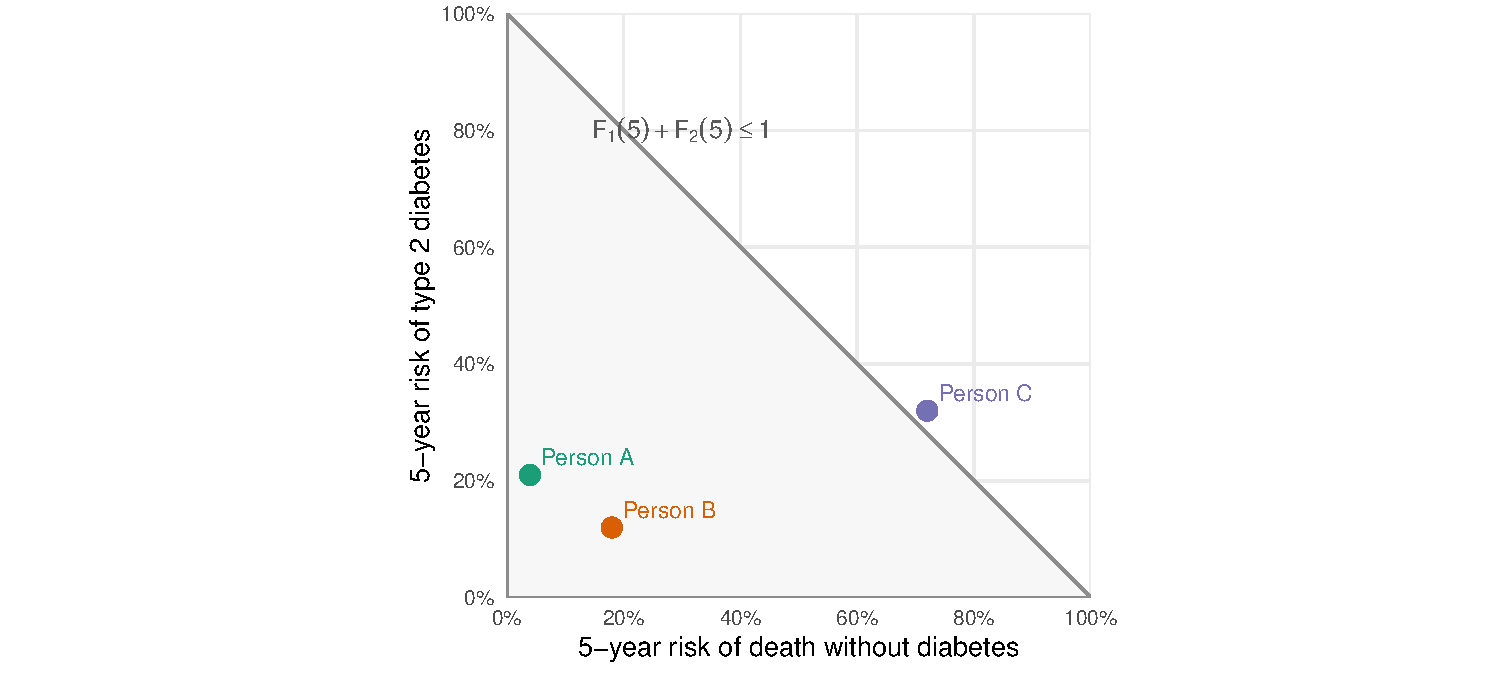
\includegraphics[width=1\textwidth]{risk-plane.pdf}
\end{center}
\end{frame}

\begin{frame}[label={sec:orgc888e88}]{Motivation}
When you estimate the cause specific risks at time \(\tau\) using semi-parametric Cox regression for the cause specific hazards, the sum of all cause specific risks can be more than 1 for certain covariate values.
\vfill
We need to export the prediction model developed in protected environments, such that we can give it to the public.
\vfill

It is unclear when to artifical censor subjects at the prediction time horizon.
\end{frame}


\begin{frame}[label={sec:org67ff19e}]{The idea: fit both risks to the prediction horizon}
Let \(Y_i(t)\) be a competing risks process with states: event-free (\(j=0\)), diabetes (\(j=1\)), or death without diabetes (\(j=2\)).

\begin{block}{Brier-score loss function}
\[
BSE=
\frac{1}{N}\sum_{i=1}^{N}w_i(\tau)\sum_{j=1}^{2}
\{F_j(\tau\mid X_i)-1\{Y_i(\tau) = j\}\}^{2}.
\]
\end{block}
\pause

\begin{itemize}
\item One loss estimates the two cause-specific models \alert{simultaneously}.
\end{itemize}

Here \(w_i(\tau)\) accounts for right censoring (without censoring, \(w_i=1\)).
\end{frame}

\section{From framework to learner}
\label{sec:org8419518}

\begin{frame}[label={sec:org7fb6385}]{Focus of this talk: a single model, not prediction strategy}
\begin{center}
Learner library $\longrightarrow$ K-fold cross-validation
$\longrightarrow$ Super Learner ensemble $\longrightarrow$ external validation
\end{center}
Candidate learners can include cause-specific Cox models, direct binomial
regression, boosting, neural networks, and constrained parametric hazard models.

\pause
\vfill

\begin{alertblock}{Focus of this talk}
One possible library member: a Cox-exponential model estimated by minimizing the Brier-score. A single learner that ensures simultaneous, coherent, and horizon-specific estimation, not
the entire prediction strategy.
\end{alertblock}
\end{frame}



\begin{frame}[label={sec:org897722d}]{The Cox-exponential model}
For causes \(j\in\{1,2\}\), assume constant baseline hazards:
\[
\lambda_j(t\mid x)=\lambda_{0j}\exp(x^\top\beta_j),\qquad \lambda_{0j}>0.
\]
Let \(A(x)=\sum_{j=1}^{2}\lambda_{0j}\exp(x^\top\beta_j)\). Then
\[
F_j(\tau\mid x)=\frac{\lambda_{0j}\exp(x^\top\beta_j)}{A(x)}
\{1-\exp[-\tau A(x)]\}.
\]

Both parameter sets \((\beta_1,\lambda_{01})\) and \((\beta_2,\lambda_{02})\) are
estimated simultaniously by minimizing the Brier score loss. The construction guarantees
\(F_1(\tau\mid x)+F_2(\tau\mid x)\leq1\) for every \(x\).
\end{frame}

\begin{frame}[label={sec:orga981c5f}]{Brier score estimation}
Assuming Cox-proportional hazards model and constant baseline hazards for all causes, our estimator becomes:

\begin{align*}
\hat{\theta}_{BSE}=&\arg\min_{\theta}\frac{1}{N}\sum_{i=1}^{N}w_i(\tau)\sum_{j=1}^{2}\\
&\{\frac{\lambda_{0j}\exp(x_i^\top\beta_j)}{A(x_i)}\{1-\exp[-\tau A(x_i)]\}-1\{Y_i(\tau) = j\}\}^{2}.
\end{align*}
\end{frame}


\begin{frame}[label={sec:orge329f73}]{Why estimate like this?}
Estimating both cause-specific hazards this way:
\begin{itemize}
\item targets calibration and discrimination directly at the prediction horizon;
\item performs well in non-proportional hazards data;
\item prevents impossible pairs of predictions;
\item produces a portable parametric learner for use outside protected enviroments.
\end{itemize}
\pause
\vfill
Choosing a simple parametric model makes sense as we only fit the model for one specific timepoint, so we don't need the baseline hazard to vary over time.
\end{frame}


\section{The role of follow-up after five years}
\label{sec:orgf993327}

\begin{frame}[label={sec:orgb0b6958}]{Artificial censoring at the prediction horizon}
Artificial censoring replaces the observed follow-up by
\[
\widetilde T_i^{(5)}=\min(\widetilde T_i,5),\qquad
\widetilde D_i^{(5)}=\widetilde D_i1\{\widetilde T_i\leq5\}.
\]
It removes all event-time information after the five-year horizon. This affects the estimates of Cox models fitted using likelihood methods.

\begin{columns}[T]
\begin{column}{0.47\textwidth}
\begin{block}{It can lose predictive power}
If proportional hazards is correct, later events inform the same $\beta_j$ that
governs hazards before five years. Discarding them wastes information.
\end{block}
\end{column}
\begin{column}{0.47\textwidth}
\begin{block}{It can gain predictive power}
If effects change after five years, an untruncated Cox fit compromises across
periods and can learn the wrong effect for the five-year target.
\end{block}
\end{column}
\end{columns}
\end{frame}


\begin{frame}[label={sec:orgd9f5dbc}]{Non-proportional hazards data}
\begin{center}
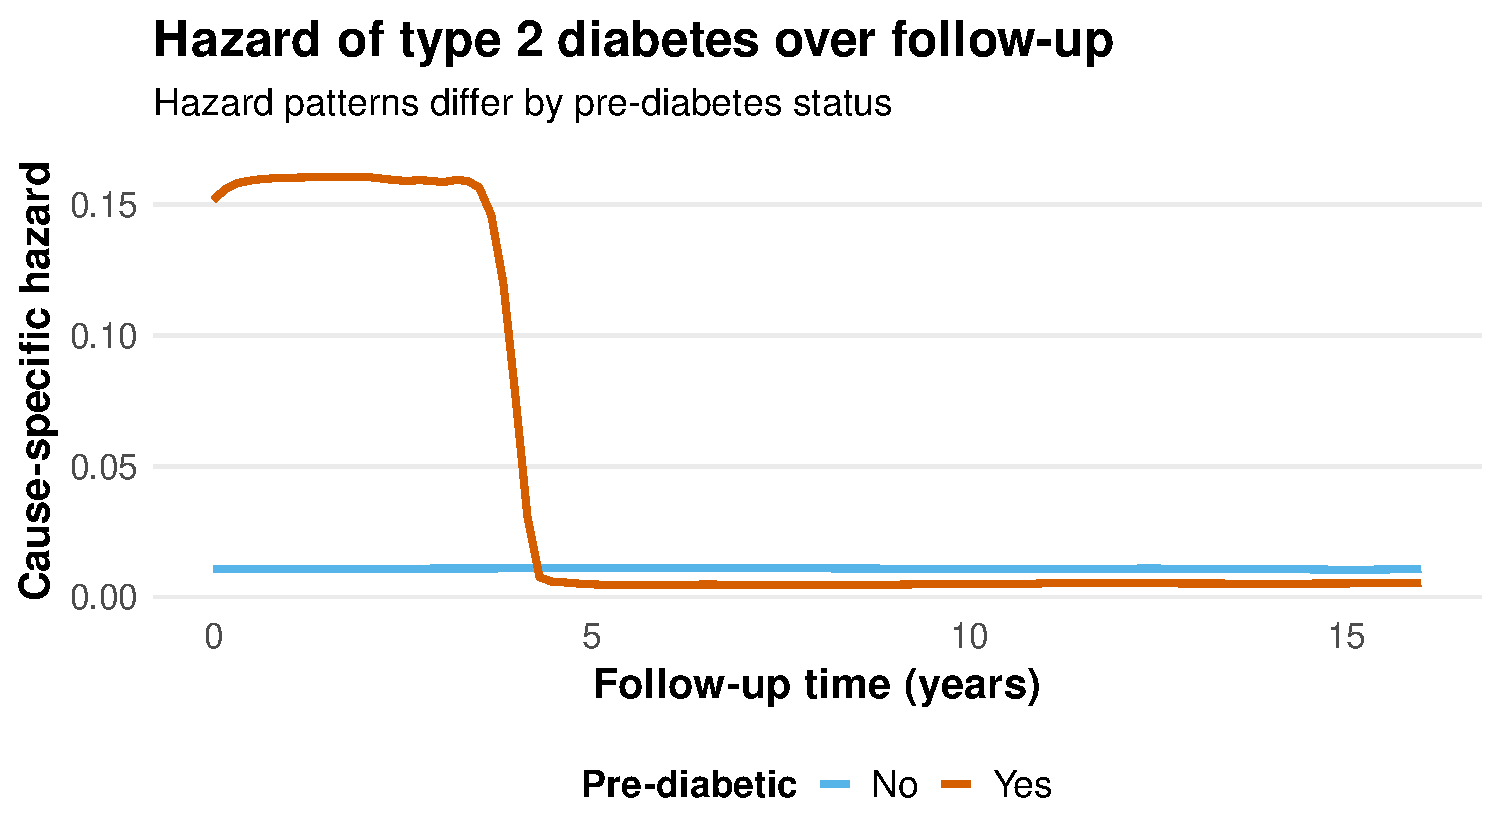
\includegraphics[width=1\textwidth]{non_prop_hazard_plot.pdf}
\end{center}
\end{frame}

\begin{frame}[label={sec:org844a52d}]{Sim study}
\begin{center}
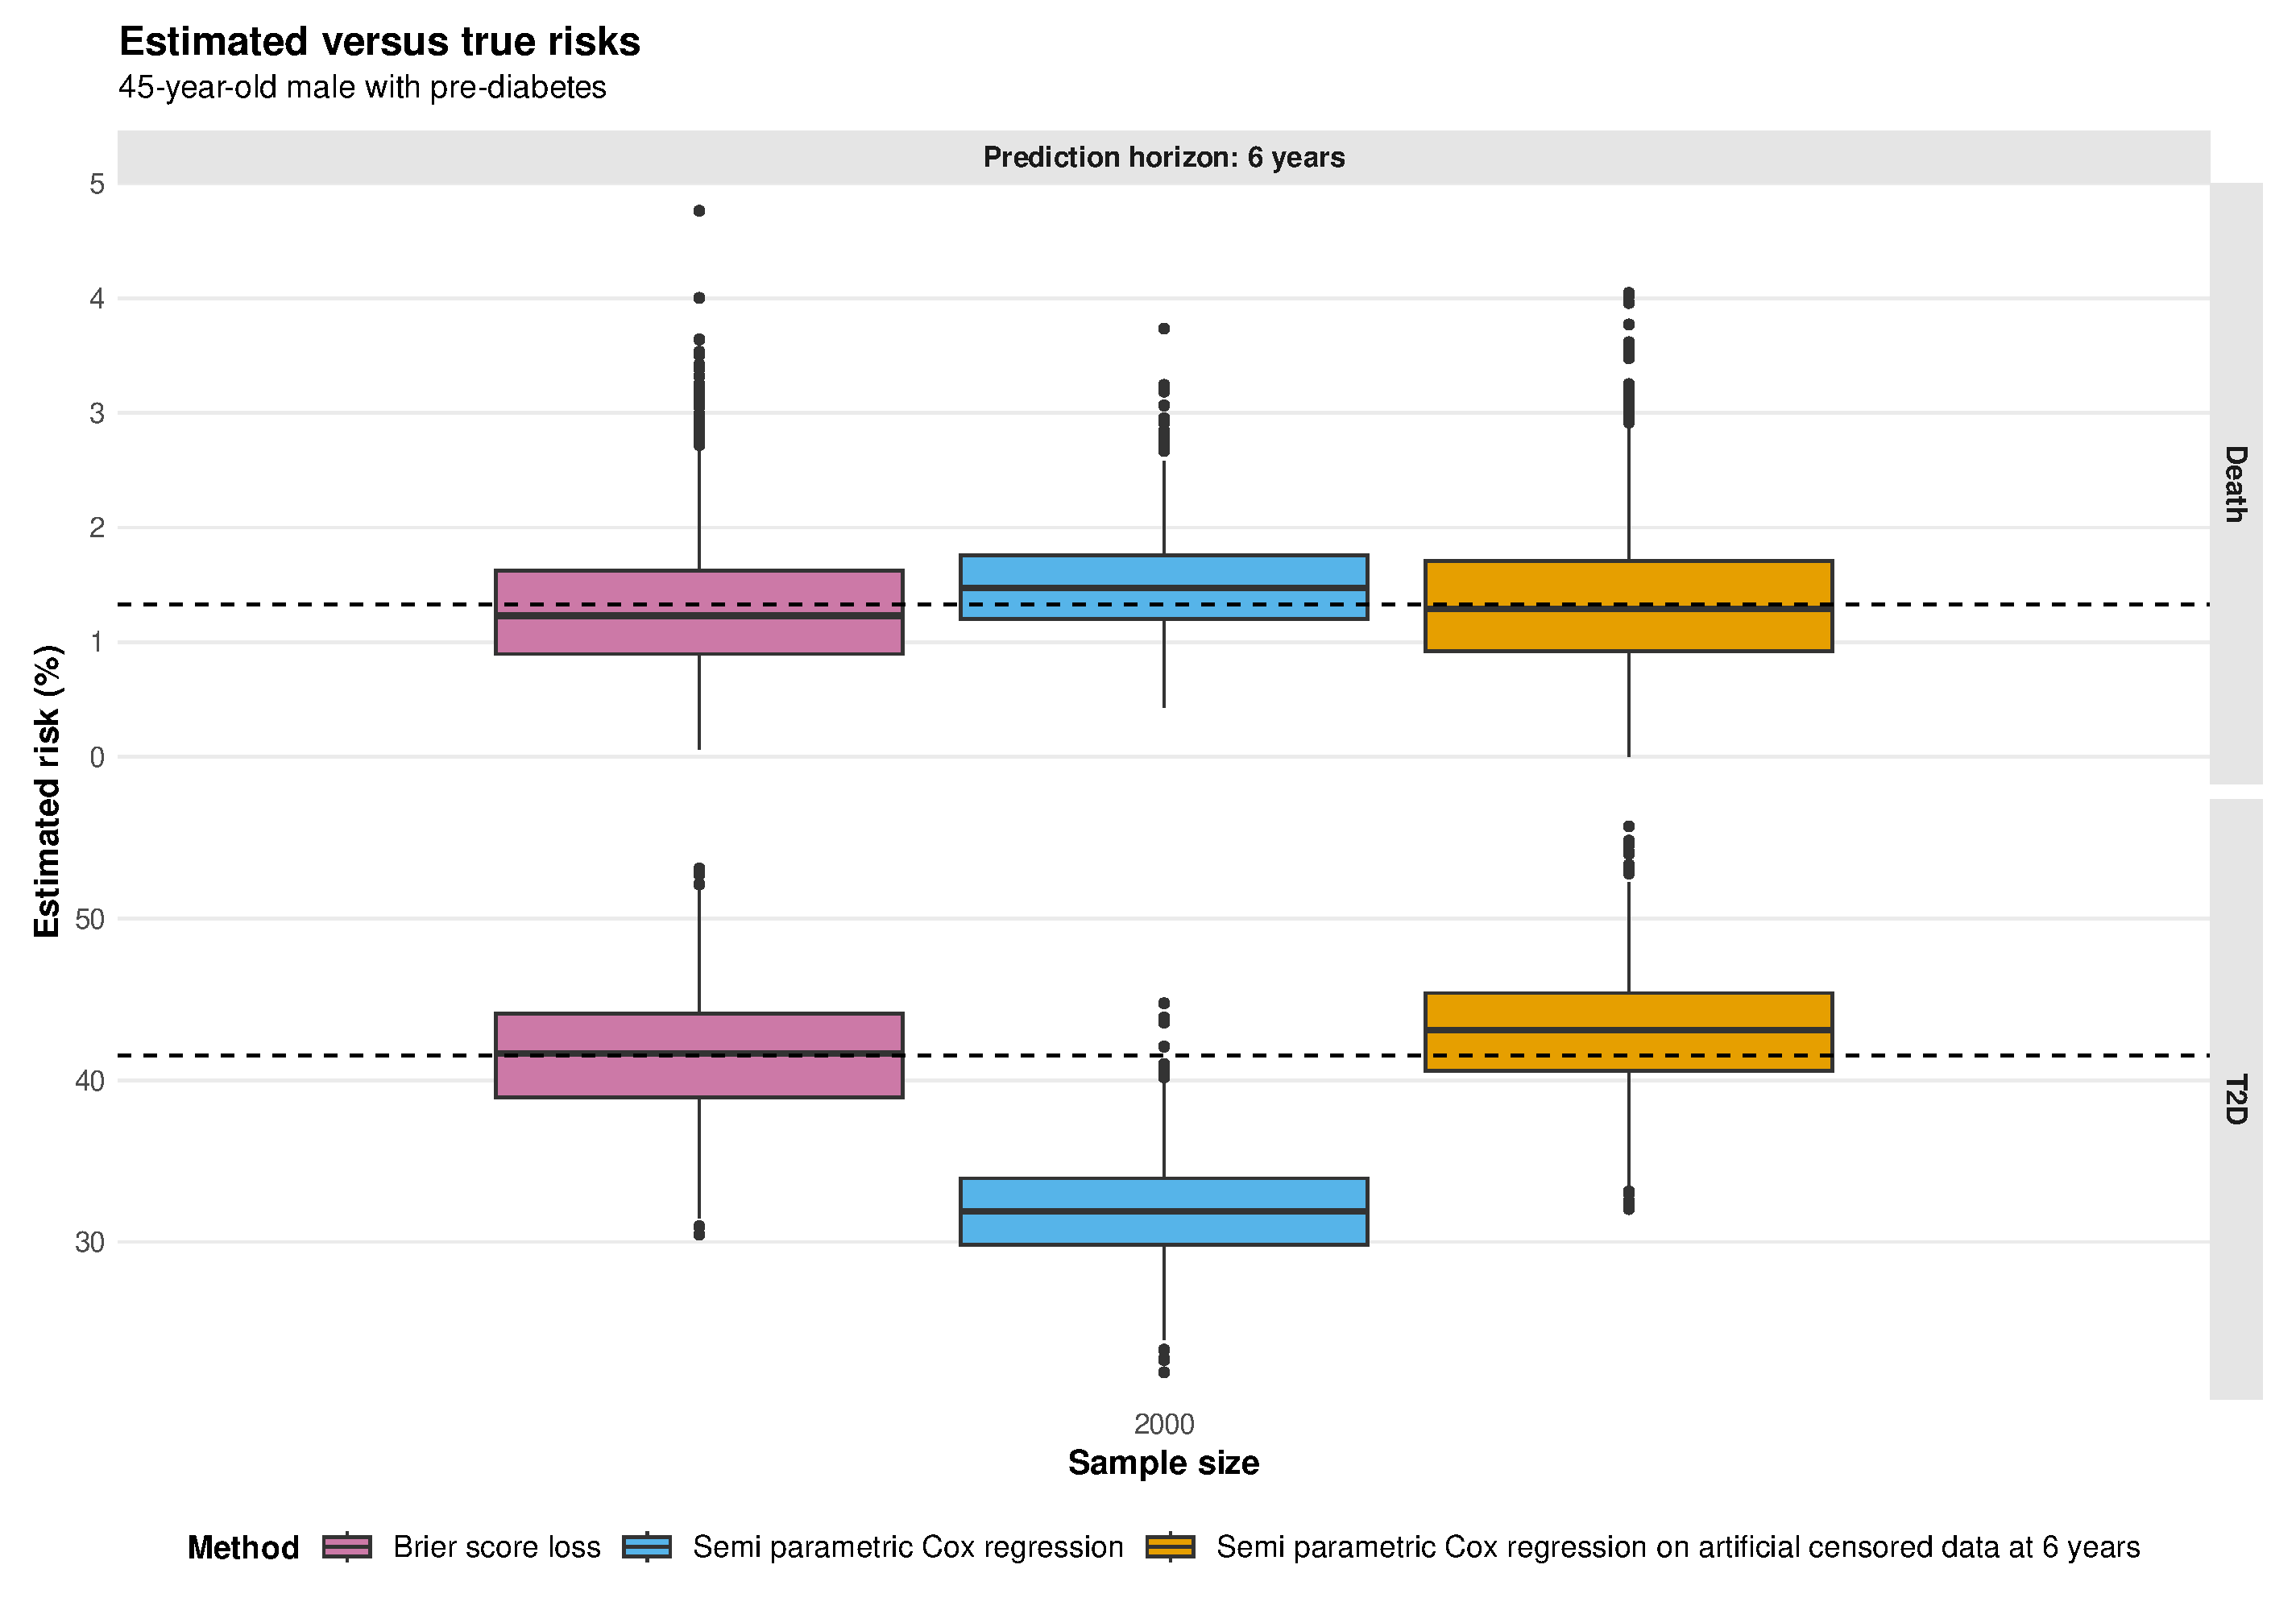
\includegraphics[width=1\textwidth]{sim_study_t6.pdf}
\end{center}
\end{frame}


\section{Application and take-home message}
\label{sec:org264e831}

\begin{frame}[label={sec:org7f2bdf4}]{Discussion}
\begin{itemize}
\item The optimization is non-convex; initialization and repeated starts matter;\pause
\item How to handle censoring; Use IPCW or fit a model for the censoring state?\pause
\item Need to extend framework to illness-death.
\end{itemize}
\end{frame}
\end{document}
